\emph{\underline{Objetivo:}}\\

El personal sanitario, dotado de un PDA, solicita la impresi\'on de un documento de un paciente que se encuentre disponible en la base de datos del hospital. Dicha impresi\'on se realizar'a por la impresora m\'as cercana al lugar en el que se ha solicitado \'esta.\\

\emph{\underline{Entradas:}} 
\begin{itemize}
\item Documento a imprimir.
\item Nombre del paciente del que solicitamos el documento a imprimir.
\end{itemize}

\emph{\underline{Precondiciones:}}\\

Los documentos que se solicitan imprimir deben encontrarse en la base de datos del hospital as'i como el paciente, que tambi'en debe estar registrado en la base de datos.\\

\emph{\underline{Salidas:}}\\

En caso de \'exito: 
\begin{itemize}
	\item Confirmaci\'on de la solicitud aceptada.
	\item Impresora por la que se va a realizar el trabajo.
	\item Documento imprimido en la impresora indicada.
\end{itemize}
En caso de fallo: 
\begin{itemize}
	\item Se informa al usuario de la imposibilidad de realizar la petici\'on.
\end{itemize}


\emph{\underline{Postcondici\'on si \'exito:}}\\

Se realiza la impresi\'on por la impresora m\'as cercana.\\

\emph{\underline{Postcondici\'on si fallo:}}\\

Se informa de que no se ha podido realizar la impresi\'on y se vuelve al men'u principal.\\

\emph{\underline{Actores: }}
\begin{itemize}
\item Usuario con PDA.
\item Servidor del hospital.
\item Cola de impresi\'on de las impresoras del centro.
\item PDA.
\end{itemize}

\emph{\underline{Secuencia normal:}} 
\begin{enumerate}
\item El usuario solicita al servidor la impresi\'on de un documento concreto de un paciente del hospital desde su PDA. Si error al conectar con el servidor pasa a E1, sino pasa a 2.
\item El servidor busca en su base de datos el documento que queremos imprimir. Si lo encuentra pasa a 3, sino pasa a E1.
\item El servidor calcula la posici\'on del PDA y en funci\'on de ella devuelve la impresora m'as cercana,  la elegida para imprimir el documento.
\item El servidor manda el documento a la cola de la impresora m\'as cercana.
\item El servidor envia al PDA la confirmaci\'on de impresi\'on aceptada, informando de cual es la impresora que en la que se realiza la tarea.
\item Volvemos al men'u principal.
\end{enumerate}

\emph{\underline{Secuencias alternativas:}}\\

E1.- Se informa al usuario de que no se puede realizar la impresi'on en ese momento y se le invita a intentarlo m\'as tarde. Volvemos al men'u principal.\\\\
\\

Para ilustrar mejor est'a secuencia de acciones, incluimos el diagrama de secuencia de este caso de uso:\\

\begin{figure*}[h!]
	\begin{center}
        		\framebox{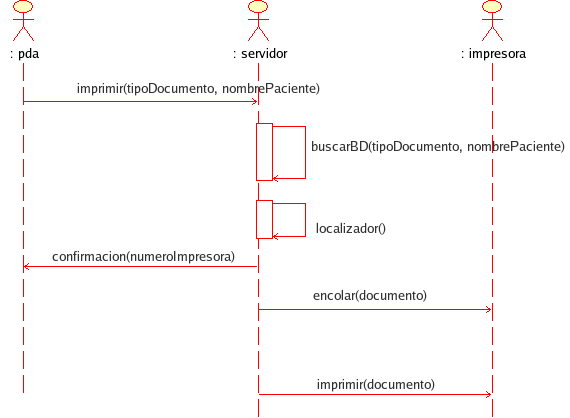
\includegraphics[width=1.0\textwidth]{dsecuenciaimprimir.png}}
     	\end{center}
    	\caption{Diagrama de secuencia de impresi'on de documentos}\label{fig:cu_imprimir}
\end{figure*}